\section{Mathematical Circuits Using the Op. Amp.: part I}

\subsection{Experiment Design}
    \subsubsection{Background}
    The operational amplifier can be used to consruct circuite to implement amplification and mathematical operations. In this experiment, we will implement six function using the combination of Op.Amp. and other components.\par

    \subsubsection{Propose}
    \begin{itemize}
        \item To verify Op.Amp. circuits for basic amplification operations
        \item To verify Op.Amp. circuits for addition/substraction
    \end{itemize}

\subsection{Experiment Design}
    \subsubsection{Materials}
        In this experiment, we will use the following components:
        \begin{itemize}
            \item Capacitors
            \item 1N4148 Diode
            \item LM741\_1 Op.Amp.
            \item Resistors
            \item Breadboard
            \item DC power supply
            \item Digital Multi-Meter
            \item Function Generator
        \end{itemize}

    \subsubsection{Circuit Diagram}
        The following circuit diagrams shows the Op.Amp. circuits for differentiation, integration, logarithm and exponential operations.
        \begin{figure}[H]
            \centering
            \begin{subfigure}{0.4\textwidth}
                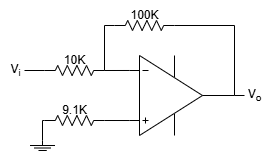
\includegraphics[width=1\linewidth]{Experiment_10/Circuit/Lab10a.drawio.png}
                \caption{Inverting Amplifier}
                \label{cir:InvAmp}
            \end{subfigure}
            \begin{subfigure}{0.4\textwidth}
                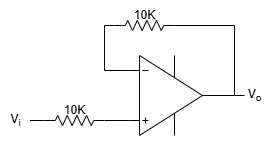
\includegraphics[width=1\linewidth]{Experiment_10/Circuit/Lab10b.drawio.png}
                \caption{Voltage Follower}
                \label{cir:VolFAmp}
            \end{subfigure}

            \begin{subfigure}{0.4\textwidth}
                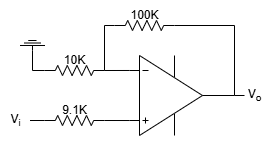
\includegraphics[width=1\linewidth]{Experiment_10/Circuit/Lab10c.drawio.png}
                \caption{Non-Inverting Amplifier}
                \label{cir:NInvAmp}
            \end{subfigure}
            \begin{subfigure}{0.4\textwidth}
                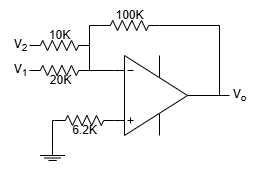
\includegraphics[width=1\linewidth]{Experiment_10/Circuit/Lab10d.drawio.png}
                \caption{Summing Amplifier}
                \label{cir:SumAmp}
            \end{subfigure}

            \begin{subfigure}{0.4\textwidth}
                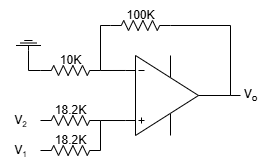
\includegraphics[width=1\linewidth]{Experiment_10/Circuit/Lab10e.drawio.png}
                \caption{Non-Inverting Summing Amplifier}
                \label{cir:NSumAmp}
            \end{subfigure}
            \begin{subfigure}{0.4\textwidth}
                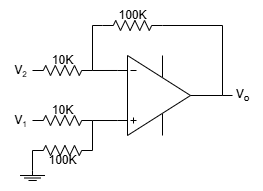
\includegraphics[width=1\linewidth]{Experiment_10/Circuit/Lab10f.drawio.png}
                \caption{Difference Amplifier}
                \label{cir:DiffAmp}
            \end{subfigure}

            \caption{Circuit Diagrams for Op.Amp. Circuits}
        \end{figure}

    \subsubsection{Theoretical Analysis}
        \begin{enumerate}[a]
            \item \textbf{Inverting Amplifier}\newline
                From the figure \ref{cir:InvAmp}, 
                we reconize this is an inverting amplifier. The output voltage can be calculated by the following equation:
                \begin{equation}
                    \frac{V_i}{R_i} = \frac{V_o}{R_{feedback}}
                \end{equation}
                Where in our circuit, the $R_i = 10k \Omega$ and $R_{feedback} = 100k \Omega$ . So plugging in the values, we get:
                \begin{equation}
                    V_o = -10V_i
                    \label{eq:InvAmp_output}
                \end{equation}

            \item \textbf{Voltage Follower}\newline
                From the figure \ref{cir:VolFAmp}, we can see that the output voltage is the same as the input voltage. So the output voltage can be calculated by the following equation:
                \begin{equation}
                    V_o = V_i
                    \label{eq:VolF_output}
                \end{equation}

                \item \textbf{Non-Inverting Amplifier}\newline
                From the figure \ref{cir:NInvAmp}, we can see that the output voltage can be calculated by the following equation:
                \begin{equation}
                    \frac{V_i}{R_i} = \frac{V_i-V_o}{R_{feedback}}
                \end{equation}
                Where in our circuit, the $R_i = 10k \Omega$ and $R_{feedback} = 100k \Omega$ . So plugging in the values, we get:
                \begin{equation}
                    V_o = 11V_i
                    \label{eq:NInvAmp_output}
                \end{equation}

            \item \textbf{Summing Amplifier}\newline
                From the figure \ref{cir:SumAmp}, we can see that the output voltage can be calculated by the following equation:
                \begin{equation}
                    \frac{V_{i1}}{R_{i1}} + \frac{V_{i2}}{R_{i2}} = \frac{V_o}{R_{feedback}}
                \end{equation}
                Where in our circuit, the $R_{i1} = 10k \Omega$, $R_{i2} = 20k \Omega$ and $R_{feedback} = 100k \Omega$ . So plugging in the values, we get:
                \begin{equation}
                    V_o = -10V_2 - 5V_1
                    \label{eq:SumAmp_output}
                \end{equation}

            \item \textbf{Non-Inverting Summing Amplifier}\newline
                From the figure \ref{cir:NSumAmp}, we can see that the output voltage can be calculated by the following equation:
                \begin{equation}
                    V_o = (10+1)V_X
                \end{equation}
                Where $V_X$ is given by the following equation:
                \begin{equation}
                    V_X = \frac{V_{i1}}{R_{i1}} + \frac{V_{i2}}{R_{i2}}
                \end{equation}
                In our circuit, the $R_{i1} = 18.2k \Omega$, $R_{i2} = 18.2k \Omega$ and $R_{feedback} = 100k \Omega$ . So plugging in the values, we get:
                \begin{equation}
                    V_o = \frac{11}{2}(V_2+V_1)
                    \label{eq:NSumAmp_output}
                \end{equation}

            \item \textbf{Difference Amplifier}\newline
                From the figure \ref{cir:DiffAmp}, we can see that the output voltage can be calculated by the following equation:
                \begin{equation}
                    \begin {aligned}
                    \frac{0-V_X}{R_{feedback}} + \frac{V_1-V_X}{R_1} = 0
                    \frac{V_2-V_X}{R_{2}} = 0 + \frac{V_X-V_O}{R_{feedback}} = 0
                    \end {aligned}
                \end{equation}
                Where in our experiment, the $R_1 = 10k \Omega$ and $R_{feedback} = 100k \Omega$ . So plugging in the values, we can slove for $V_O$:
                \begin{equation}
                    V_O = 10V_1 - 10V_2
                    \label{eq:DiffAmp_output}
                \end{equation}
        \end{enumerate}

\subsection{Experiment record}
    \subsubsection{The Inverting Amplifier}
    \begin{enumerate}[I]
        \item \textbf{Data Recorded}\newline
            The recorded data for the integration operation circuit is shown in the following table:
            \begin{table}[H]
                \centering
                \begin{tabular}{l|rrrrrrrr}
                \toprule
                $V_i$ & 0.10  & 0.30  & 0.50  & 0.70  & 0.90  & 1.10  & 1.30  & 1.50 \\
                \midrule
                $V_o$ (Mea) & -1.00 & -3.05 & -5.09 & -7.11 & -9.16 & -11.15 & -11.36 & -11.36 \\
                \midrule
                $V_o$ (Theo) & -1.00 & -3.00 & -5.00 & -7.00 & -9.00 & -11.00 & -13.00 & -15.00 \\
                Error & 0.00\% & 0.03\% & 0.03\% & 0.02\% & 0.03\% & 0.02\% & 1.59\% & 5.89\% \\
                \bottomrule
                \end{tabular}%
                \caption{Recorded Data for the Inverting Amplifier}
                \label{tab:InvAmp}
            \end{table}
        \item \textbf{Data Analysis}\newline
            The theoretical output voltage for the inverting amplifier is calculated by the equation \ref{eq:InvAmp_output}. And the square error between the measured and theoretical output voltage is calculated and shown in the table \ref{tab:InvAmp}.\par
            
            Reading the table, we can see that the error between the measured and theoretical output voltage is small, so our circuit is working as expected. And we can notice the ouput voltage is bound to the maximum value of 11.36V, which is the value of the reference voltage.\par
    \end{enumerate}
    
    \subsubsection{The Voltage Follower}
    \begin{enumerate}[I]
        \item \textbf{Data Recorded}\newline
            The recorded data for the integration operation circuit is shown in the following table:
            \begin{table}[H]
                \centering
                \begin{tabular}{l|rrrrrrrr}
                    \toprule
                    $V_i$ & 0.100 & 0.300 & 0.500 & 0.700 & 0.900 & 1.100 & 1.300 & 1.500 \\
                    \midrule
                    $V_o$ (Mea) & 0.091 & 0.299 & 0.499 & 0.695 & 0.896 & 1.096 & 1.296 & 1.498 \\
                    \midrule
                    $V_o$ (Theo) & 0.100 & 0.300 & 0.500 & 0.700 & 0.900 & 1.100 & 1.300 & 1.500 \\
                    Error & 0.81\% & 0.00\% & 0.00\% & 0.01\% & 0.00\% & 0.00\% & 0.00\% & 0.00\% \\
                    \bottomrule
                    \end{tabular}%
                    \caption{Recorded Data for the Voltage Follower}
                    \label{tab:VolFAmp}
            \end{table}
        \item \textbf{Data Analysis}\newline\
            The theoretical output voltage for the voltage follower is calculated by the equation \ref{eq:VolF_output}. And the square error between the measured and theoretical output voltage is calculated and shown in the table \ref{tab:VolFAmp}.\par

            From the table, we can notice the error is very small. This shows our circuit is working as expected. And because the output voltage is below the reference voltage, there were no saturation as was in the last experiment.\par
    \end{enumerate}

    \subsubsection{The Non-Inverting Amplifier}
    \begin{enumerate}[I]
        \item \textbf{Data Recorded}\newline
            The recorded data for the integration operation circuit is shown in the following table:
            \begin{table}[H]
                \centering
                \begin{tabular}{l|rrrrrrrr}
                    \toprule
                    $V_i$ & 0.10  & 0.30  & 0.50  & 0.70  & 0.90  & 1.10  & 1.30  & 1.50 \\
                    \midrule
                    $V_o$ (Mea) & 1.09  & 3.32  & 5.51  & 7.76  & 10.02 & 10.64 & 10.64 & 10.64 \\
                    \midrule
                    $V_o$ (Theo) & 1.10  & 3.30  & 5.50  & 7.70  & 9.90  & 12.10 & 14.30 & 16.50 \\
                    Error & 0.01\% & 0.00\% & 0.00\% & 0.01\% & 0.01\% & 1.46\% & 6.55\% & 12.61\% \\
                    \bottomrule
                    \end{tabular}%
                    \caption{Recorded Data for the Non-Inverting Amplifier}
                    \label{tab:NInvAmp}
            \end{table}
        \item \textbf{Data Analysis}\newline
            The theoretical output voltage for the non-inverting amplifier is calculated by the equation \ref{eq:NInvAmp_output}. And the square error between the measured and theoretical output voltage is calculated and shown in the table \ref{tab:NInvAmp}.\par

            From the table, we can notice the error is small. This shows our circuit is working as expected. And we can notice the ouput voltage is bound to the maximum value of 10.64V, which is about the value of the reference voltage 11V.\par
    \end{enumerate}

    \subsubsection{The Summing Amplifier}
    \begin{enumerate}[I]
        \item \textbf{Data Recorded}\newline
            The recorded data for the integration operation circuit is shown in the following table:
            \begin{table}[H]
                \centering
                \begin{tabular}{l|rrrr}
                    \toprule
                    $V_1$ & 0.10  & 0.50  & 0.10  & 1.00 \\
                    $V_2$ & 0.20  & 0.10  & 0.50  & 0.40 \\
                    \midrule
                    $V_o$ (Mea) & -2.05 & -3.52 & -5.58 & -11.36 \\
                    \midrule
                    $V_o$ (Theo) & -2.50 & -3.50 & -5.50 & -9.00 \\
                    Error & 3.20\% & 0.00\% & 0.02\% & 6.89\% \\
                    \bottomrule
                    \end{tabular}
                \caption{Recorded Data for the Summing Amplifier}
                \label{tab:SumAmp}
            \end{table}
        \item \textbf{Data Analysis}\newline
            The theoretical output voltage for the summing amplifier is calculated by the equation \ref{eq:SumAmp_output}. And the square error between the measured and theoretical output voltage is calculated and shown in the table \ref{tab:SumAmp}.\par

            From the table, we can notice the error is small. This shows our circuit is working as expected.\par
    \end{enumerate}

    \subsubsection{The Non-Inverting Summing Amplifier}
    \begin{enumerate}[I]
        \item \textbf{Data Recorded}\newline
            The recorded data for the integration operation circuit is shown in the following table:
            \begin{table}[H]
                \centering
                \begin{tabular}{|l|rrrr|}
                    \toprule
                    $V_1$ & 0.100 & 0.500 & 0.800 & 1.000 \\
                    $V_2$ & 0.200 & 0.300 & 0.500 & 1.000 \\
                    \midrule
                    $V_o$ (Mea) & 1.640 & 4.439 & 7.205 & 10.638 \\
                    \midrule
                    $V_o$ (Theo) & 1.650 & 4.400 & 7.150 & 11.000 \\
                    Error & 0.00\% & 0.01\% & 0.01\% & 0.11\% \\
                    \bottomrule
                    \end{tabular}%
            \caption{Recorded Data for the Non-Inverting Summing Amplifier}
            \label{tab:NSumAmp}                    
            \end{table}
        \item \textbf{Data Analysis}\newline
            The theoretical output voltage for the non-inverting summing amplifier is calculated by the equation \ref{eq:NSumAmp_output}. And the square error between the measured and theoretical output voltage is calculated and shown in the table \ref{tab:NSumAmp}.\par

            From the table, we can notice the error is small. This shows our circuit is working as expected. Note at the last data, the output is limited to 10.638V, which's around the voltage of the reference voltage 11V.\par
    \end{enumerate}

    \subsubsection{The Difference Amplifier}
    \begin{enumerate}[I]
        \item \textbf{Data Recorded}\newline
            The recorded data for the integration operation circuit is shown in the following table:
            \begin{table}[H]
                \centering
                \begin{tabular}{|l|rrr|}
                    \toprule
                    $V_1$ & 0.10  & 0.50  & 1.00 \\
                    $V_2$ & 0.40  & 0.10  & 0.40 \\
                    \midrule
                    $V_o$ (Mea) & -3.18 & 4.16  & 6.17 \\
                    \midrule
                    $V_o$ (Theo) & -3.00 & 4.00  & 6.00 \\
                    Error & 0.36\% & 0.15\% & 0.08\% \\
                    \bottomrule
                    \end{tabular}%
                \caption{Recorded Data for the Difference Amplifier}
                \label{tab:DiffAmp}
            \end{table}

        \item \textbf{Data Analysis}\newline
            The theoretical output voltage for the difference amplifier is calculated by the equation \ref{eq:DiffAmp_output}. And the square error between the measured and theoretical output voltage is calculated and shown in the table \ref{tab:DiffAmp}.\par

            From the table, we can notice the error is small. This shows our circuit is working as expected.\par
    \end{enumerate}


\subsection{Experiment Conclusion}
    \subsubsection{Conclusion}
        In this experiment, we have implemented six mathematical operations using the Op.Amp. circuits. The output voltage of the circuits were calculated and compared with the theoretical output voltage. The error between the measured and theoretical output voltage was calculated and analyzed. From the analysis, we can conclude that the circuits are working as expected.\par